\section{Removal Methods and Detector Models}
\label{sec:methods}

All removal methods start from the poisoned model $f$ except the two retraining
methods, which start from random initialisation. The post-training methods use
SGD with momentum 0.9 and weight decay $5\times10^{-4}$, and are deliberately
kept simple: the goal is to compare families under a common budget, not to tune
each family to its best. The CIFAR-10 settings common to all runs are listed in
Table~\ref{tab:protocol}.

\subsection{Deletion and Retraining}
\method{Retrain}$_{\setminus F}$ is the reference deletion method: train a new
network from scratch on $\mathcal{D}\setminus\fset$ with the full twelve-epoch
schedule. It is expensive, but it is the method that the oracle literature
reports as a success, and it isolates the effect of the forget set from any
property of the poisoned initialisation. When $\fset$ equals the true poison
set, this is the gold model.

\subsection{Fine-Tuning on the Retained Set}
\method{Fine-tune} continues training the poisoned model for three epochs at
learning rate $0.01$ on $\mathcal{D}\setminus\fset$. It is the cheapest possible
response to a detector and is common in practice when retraining is not
affordable. It has no mechanism for forgetting: it only reinforces the retained
data.

\subsection{Gradient Ascent and SCRUB}
\method{NegGrad+} performs three epochs of ascent on the cross-entropy of the
forget set, balanced by descent on a matched random batch from the retained set,
at learning rate $10^{-3}$ \cite{amnesiac}. \method{SCRUB} first fine-tunes a
teacher on the retained set for three epochs, then trains a student for three
epochs to minimise cross-entropy on the retained set plus a Kullback--Leibler
term that pulls the student's distribution on the forget set towards the
teacher's \cite{scrub}. Both methods are designed for exact forget sets; the
grid tests how they behave when the set is noisy.

\subsection{Repair and Inoculation}
The recipe is the only method in the suite that is designed around an imperfect
forget set. It has two stages.

\emph{Label repair.} Features are extracted from the penultimate layer of the
poisoned model for all training samples. Each flagged sample receives a
pseudo-label by a weighted $k$-nearest-neighbour vote ($k{=}10$,
inverse-distance weights) over the \emph{unflagged, non-target} training data.
The sample is kept, not deleted, with its repaired label. The intuition is that
a poisoned image whose patch is ignored looks like its true class, so the
nearest neighbours in feature space are clean images of that class rather than
of the target class.

\emph{Inoculation.} A pool of 5{,}000 retained samples that the poisoned model
does not confidently classify as the target class is trigger-stamped and kept
with its true label. Each mini-batch is composed of 60\% retained samples, 20\%
flagged samples with pseudo-labels, and 20\% inoculated samples. The network is
fine-tuned for three epochs at learning rate $0.01$. Presenting the trigger with
the correct label teaches the network that the trigger is not predictive of the
target class, which is the mechanism by which the recipe can tolerate poison
that the forget set missed. Fig.~\ref{fig:recipe} draws the two streams and where
they meet.

\begin{figure}[t]
\centering
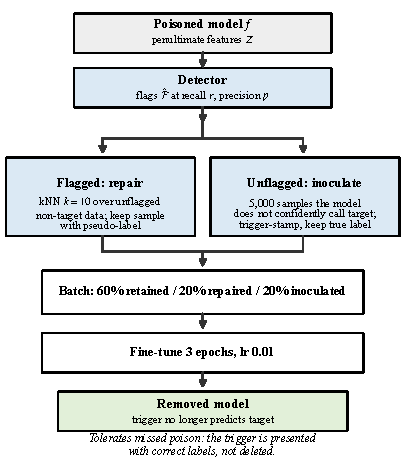
\includegraphics[width=0.92\columnwidth]{fig14_recipe_pipeline.pdf}
\caption{The repair-and-inoculate recipe. Flagged samples are relabelled by a
$k$-nearest-neighbour vote over unflagged, non-target data; unflagged samples
supply the trigger-stamped inoculation pool. The streams are mixed 60/20/20 and
fine-tuned for three epochs. The lower branch is what tolerates missed poison:
the trigger is presented with correct labels rather than deleted.}
\label{fig:recipe}
\end{figure}

\emph{Inoculation only.} To separate the two stages we also run an
inoculation-only variant that keeps the entire training set, applies no label
repair, and fine-tunes with 20\% trigger-stamped samples for three epochs. This
is the F-independent baseline of the E1 grid: it uses no forget set at all and
therefore cannot degrade with detector recall, but it also cannot repair the
poisoned labels. A second variant replaces the true trigger with a synthesised
one (Section~\ref{sec:general}).

\subsection{Trigger Synthesis}
The synthesis baseline follows Neural Cleanse \cite{nc}. For each class other
than the target, a soft mask $m\in[0,1]^{32\times32}$ and a pattern are optimised
for 200 Adam steps at learning rate $0.1$ on 64 samples of that class, with the
objective of driving the model to the target class while penalising the mask
mass with weight $10^{-3}$. The class with the smallest mask mass is retained as
the estimated trigger. The overlap with the true patch is measured by
intersection over union (IoU) after thresholding the mask at $0.5$. The
synthesised trigger is then used wherever the true trigger would be used, both
for inoculation and as the proxy in Calibrate-then-Remove.

\subsection{Calibrate-then-Remove}
Calibrate-then-Remove (CaR) is our attempted mechanism for turning detector
output into a removal decision with a guarantee. For a grid of spectral-signature
thresholds $\theta$, it forms the corresponding forget set, applies the recipe's
repair stage to obtain a proxy-removed model, and measures the proxy model's
response $\tau$ to the \emph{synthesised} trigger. If a threshold yields
$\tau\leq5\%$, the same threshold is applied to the real test trigger and the
removal is accepted. If no threshold qualifies, the method falls back to the
F1-optimal threshold. The logic is conformal in spirit: the synthesised trigger
plays the role of a calibration sample that is exchangeable with the test
trigger \cite{vovk,angelopoulos}. It fails if the synthesised trigger is not a
valid proxy, which is what we observe.

\subsection{Amplify-and-Detect}
The second attempted mechanism tests a hypothesis rather than a pipeline: that
partial unlearning makes the poison it failed to remove easier to detect, because
the network must reallocate the trigger association onto the residual poison and
therefore represents it more sharply. We operationalise it by applying partial
label repair at two strengths, then fitting a detector to separate the missed
poison from clean target-class data and measuring AUC \eqref{eq:auc}. The
pre-registered promotion gate required an AUC gain of at least $+0.10$ over the
base model, a clean-accuracy loss of at most two points, and a gain larger than a
matched clean-removal control that receives the same intervention on clean data
instead of poison. All three clauses had to hold on all seeds.

\subsection{Detectors}
We use two published detectors, both applied to the penultimate features of the
poisoned model.

\emph{Activation clustering} \cite{ac} processes each class separately: it
projects the class's features to ten principal components, runs $k$-means with
$k{=}2$, and flags the smaller cluster if its size fraction is below 0.35 and
the silhouette score exceeds 0.10.

\emph{Spectral signatures} \cite{ss} computes, for each class, the top singular
vector of the centred feature matrix and scores every sample by the squared
projection onto that direction. It flags a fixed budget of $1.5N_p$ samples with
the largest scores. The fixed budget is why its precision degrades at low poison
rates: at a 1\% poison rate the budget is 750 samples for 500 true poison, and at
5\% it is 3{,}750 for 2{,}500.

Fig.~\ref{fig:detpipeline} draws the two pipelines side by side. Both read the
same penultimate features and differ only in how they score a sample; the two
annotations mark the failure modes that recur in the grid, an empty flag set at
10\% poison for activation clustering and a 33.8\% recall at 1\% for spectral
signatures.

\begin{figure*}[t]
\centering
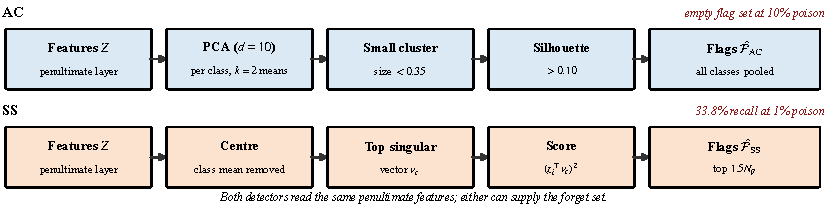
\includegraphics[width=\textwidth]{fig12_detection_pipeline.pdf}
\caption{The two detectors as pipelines. Both read the same penultimate
features. Activation clustering (top) returns no flags at a 10\% poison rate;
spectral signatures (bottom) recovers 33.8\% of the poison at a 1\% rate because
its fixed $1.5N_p$ budget lets clean samples crowd out poison.}
\label{fig:detpipeline}
\end{figure*}

Both detectors were also run on VGG-16-BN and MobileNetV2 models. Those runs were
degenerate (no flags, or flags with no true positives) and are excluded from the
tables; we report the ResNet-18 operating points, which are the ones that
produce non-trivial forget sets.

\subsection{Efficiency-Oriented Baselines}
Two further baselines are included for completeness. SISA-5 shards the training
set into five parts, trains one model per shard, and unlearns by retraining the
shards that contain forget-set samples \cite{sisa}; we report both the
oracle-recall variant and a recall-0.5 variant. Fine-pruning removes filters
with the smallest average activation on clean data, in increasing fractions
\cite{finepruning}. These methods are not swept over the grid because their
compute profile is different, but they answer the natural question of whether a
cheaper mechanism can substitute for deletion.

\subsection{What Each Family Needs}
Fig.~\ref{fig:families} arranges the families by what they consume. Deletion is
the only method that never touches the poisoned weights; it discards the network
and pays a full schedule. Fine-tuning and the two ascent methods all start from
the poisoned model and differ only in how they use $\fset$, and all three assume
that $\fset$ is the poison, which is the assumption the grid relaxes. The recipe
is the only family that consumes the trigger, and that is the asymmetry the
figure is meant to make visible: trigger knowledge buys tolerance to an
incomplete $\fset$, and nothing else in the suite has it. The compute column
also explains why the efficiency-oriented methods are evaluated separately
rather than inside the grid: deletion buys its clean removal with a full
schedule, while the three-epoch methods are cheap precisely because they stay
close to the poisoned model.

\begin{figure*}[t]
\centering
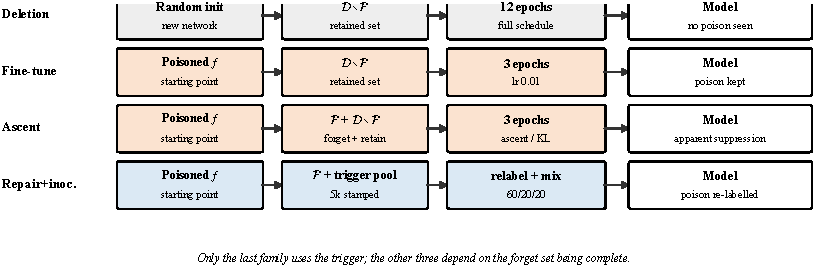
\includegraphics[width=\textwidth]{fig13_removal_families.pdf}
\caption{The four removal families and what each consumes. Only the
repair-and-inoculation family uses the trigger; the other three assume that the
forget set is the poison. The last column states the intended mechanism, not the
measured outcome.}
\label{fig:families}
\end{figure*}
